\begin{infocard}{Enlace covalente}
    Los \textbf{enlaces covalentes} se forman cuando dos átomos comparten pares de electrones.
    \begin{figure}[H]
        \centering
        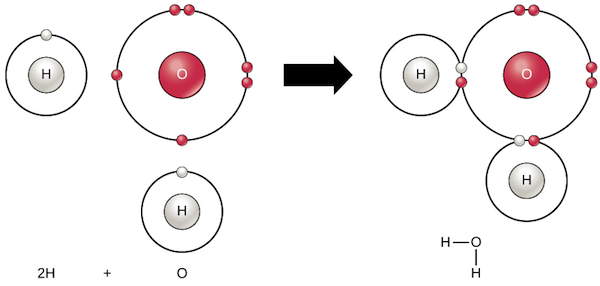
\includegraphics[width=\linewidth]{../images/2e56e620e79858d5dca7103b22dbde6eb5c52f0c}
        % \caption{Átomos de hidrógeno que comparten electrones con un átomo de oxígeno para formar enlaces covalentes al crear una molécula de agua.}
        % \label{fig:enlace_covalente}
    \end{figure}

    Estos enlaces son más comunes que los enlaces iónicos en las moléculas de los organismos vivos.
\end{infocard}